%% Los cap'itulos inician con \chapter{T'itulo}, estos aparecen numerados y
%% se incluyen en el 'indice general.
%%
%% Recuerda que aqu'i ya puedes escribir acentos como: 'a, 'e, 'i, etc.
%% La letra n con tilde es: 'n.

\chapter{Estado del Arte}

A lo largo de este cap\'itulo se explica el punto m\'as avanzado en que se encuentra hoy en d\'ia los SIG y los servidores de mapas, haciendo incapi\'e en aquellos que implementan mapas tem\'aticos, sin pasar por alto la interfaz de usuario que utilizan para la configuraci\'on de servidor. Por \'ultimo, basado en la investigaci\'on de las herramientas existentes que utilizan mapas tem\'aticos y de la interfaz visual para su configuraci\'on, se decide la mejor estrategia para utilizar sobre el servidor. No sin antes acercar al lector a la historia del origen y evoluci\'on de los mapas tem\'aticos.


\section{Origen y evoluci\'on de los mapas tem\'aticos}

Claudio Tolomeo (siglo II), griego o egipcio, es mejor conocido como el astr\'onomo autor de la idea err\'onea del Universo, sostenida durante catorce siglos, seg\'un la cual la Tierra ocupa el centro y los planetas giran a su alrededor. Sin embargo, el gran m\'erito de Tolomeo radica en la geograf\'ia.

Los mapas tem\'aticos tienen su antecedente en Tolomeo, quien los elabor\'o de tipo hist\'orico. En forma aislada aparecieron desde el siglo XVIII mapas espec\'ificos para representar alg\'un fen\'omeno de la naturaleza, adem\'as de los hist\'oricos que fueron los m\'as comunes. En la segunda mitad de este siglo se popularizaron los t\'erminos mapa y cartograf\'ia tem\'aticos y, en esta \'epoca, se han multiplicado en grado superlativo. Los primeros mapas tem\'aticos fueron muy simples, sin embargo, ameritaron su publicaci\'on en las revistas geol\'ogicas de mayor prestigio, aunque presentaban una informaci\'on muy general y pobre en extremo, nadie puede negar el inmenso valor de esa informaci\'on.\cite{histTematico}

Si los mapas alcanzan un grado, digamos cercano a la perfecci\'on, puede pensarse que el tema de investigaci\'on queda clausurado. Esto es cierto s\'olo parcialmente. En la medida que los mapas que representaban rasgos f\'isicos de la superficie terrestre se fueron perfeccionando, surgi\'o la necesidad de expresar otros fen\'omenos y objetos: los suelos, las comunidades de flora y fauna, las rocas, los climas, la estructura profunda de la Tierra. De la cartograf\'ia general se pas\'o a la tem\'atica.

El mapa ha sido siempre un reflejo del estado de desarrollo de determinadas disciplinas cient\'ificas. Si actualmente hay decenas o cientos de mapas tem\'aticos diversos, esto da una idea del estado actual de las geociencias. Uno de los m\'as conocidos es el publicado en 1936 sobre la agricultura de Estados Unidos. Destac\'o por su originalidad. Posteriormente han sido editados mapas complejos en diversos pa\'ises, resultado de investigaciones prolongadas e incluso multidisciplinarias, apoyadas por instituciones cient\'ificas y financieras.

Los mapas tem\'aticos de un mismo pa\'is o regi\'on se hacen peri\'odicamente, pretenden que la informaci\'on contenida en el mismo sea f\'acilmente comprendida por el lector o usuario. Si esta es correcta y valiosa, pero mal expresada por no usar los colores o s\'imbolos adecuados, la lectura del mapa se vuelve labor tortuosa. Por esto, el dise\~no final queda a cargo de un especialista altamente calificado, quien define colores, s\'imbolos, tama\~nos de letras, grosor de l\'ineas, distribuci\'on de la leyenda y otros problemas semejantes. Es la parte art\'istica de la cartograf\'ia. \cite{histTematico}

En los \'ultimos quince a\~nos asistimos a una aut\'entica revoluci\'on en el amplio campo de la cartograf\'ia, y muy especialmente en la caracterizaci\'on tridimensional del territorio. Se ha pasado en unas d\'ecadas de una cartograf\'ia casi secreta, en manos de los ej\'ercitos o de los estados, y muy limitada, a una enorme disponibilidad e incluso a la gratuidad de los materiales. Con el tiempo se han creado servidores que facilitan cartograf\'ia tem\'atica a cualquier usuario. Los servidores permiten visualizar mapas, la localizaci\'on, la identificaci\'on de atributos, las consultas sencillas e incluso la conexi\'on a bases de datos remotas para poder crear mapas tem\'aticos. \cite{sigTematico}



\section{Herramientas SIG que implementan mapas tem\'aticos}

Hoy en d\'ia existen servicios en l\'inea que son capaces de generar mapas tem\'aticos a partir de ciertos par\'ametros de entrada. Sin embargo es peque\~na la cantidad de t\'ecnicas de representaci\'on de datos estad\'isticos que se pueden manejar, en general los datos estad\'isticos y geogr\'aficos disponibles son los que se encuentran en los servidores de quienes administran el servicio y, en la mayor\'ia de los casos, su c\'odigo no puede ser descargado ni modificado de acuerdo a las necesidades de los usuarios. Existen herramientas de escritorio y, adem\'as, plataformas que usan servidores de mapas, lo cuales cuentan con m\'odulos que permiten la creaci\'on de mapas tem\'aticos y dejan al usuario utilizar los datos estad\'isticos que posee, sin embargo, estas son aplicaciones que no se centran en el trabajo con mapas tem\'aticos, sino en la edici\'on y gesti\'on de datos geogr\'aficos por lo que en su mayor\'ia el n\'umero de t\'ecnicas de representaci\'on de datos estad\'isticos con el que se trabaja no es muy amplio; adem\'as, en no todos los casos el c\'odigo fuente est\'a disponible.


\subsection{QGis}
QGis es un sistema de informaci\'on geogr\'afica de software libre\footnote{significa que los usuarios tienen la libertad de ejecutar, copiar, distribuir, estudiar, modificar y mejorar el software} y de c\'odigo abierto\footnote{software cuyo c\'odigo fuente se ha puesto a disposici\'on de todo el mundo de manera gratuita}, multiplataforma, que funciona junto con un servidor web \cite{ART}. Esta herramienta cuenta con un peque\~no m\'odulo para crear mapas tem\'aticos. La ayuda del software hace una descripci\'on acerca del uso de los mismos, en esta se plantea que est\'an disponibles cuatro modos para crear diferentes tipos de estos mapas.

Como ventajas, este sistema multiplataforma de c\'odigo abierto presenta funcionalidades para la creaci\'on de los mapas tem\'aticos, que permiten seleccionar, en un men\'u deplegable, varias opciones; la que nos concierne es la de Categorized, que permite asignar un color diferente a cada capa, y as\'i, crear un mapa tem\'atico, donde separa por colores la informaci\'on pertinente a estas (figura \ref{qGisTematic}). 

\begin{wrapfigure}{l}{0.5\textwidth}
\vspace{-20pt}
\begin{center}
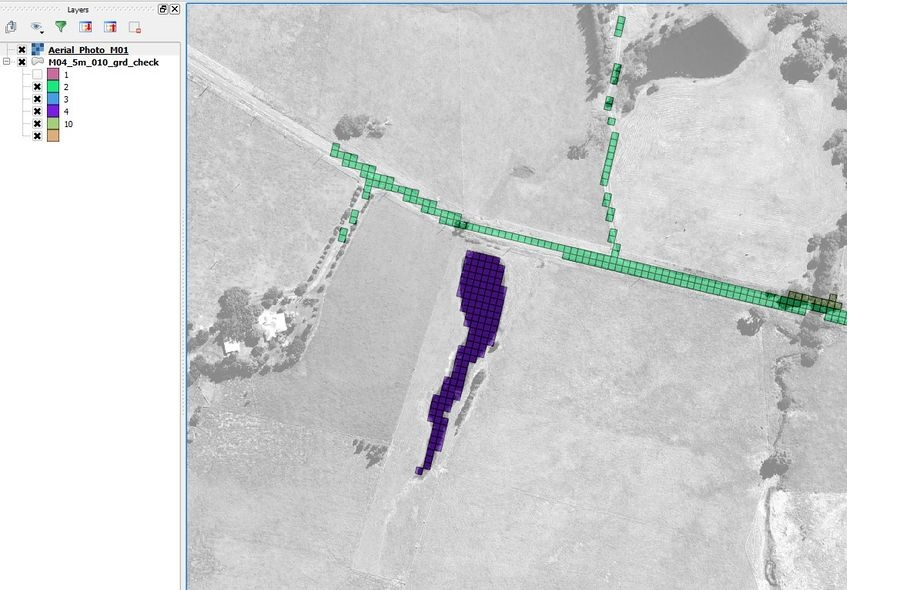
\includegraphics[width=0.52\textwidth]{images/qGisTematic.jpg} 
\end{center} \vspace{-20pt} \caption{Mapa tem\'atico creado con QGis.}  \label{qGisTematic} \vspace{-10pt} 
\end{wrapfigure}

Adem\'as, una de las mayores ventajas de esta herramienta es la posibilidad de usar Quantum GIS como GUI (Interfaz gr\'afica de usuario) del SIG GRASS \cite{qgis}, utilizando toda la potencia de an\'alisis de este \'ultimo en un entorno de trabajo m\'as amigable (figura \ref{qGisvisual}). QGIS est\'a desarrollado en C++\footnote{lenguaje de programaci\'on multiparadigma dise\~nado en 1979 por Bjarne Stroustrup.}, usando la biblioteca Qt\footnote{framework multiplataforma orientado a objetos ampliamente usado para desarrollar programas que utilicen interfaz gr\'afica de usuario} para su Interfaz gr\'afica de usuario.

A pesar de las ventajas expuestas, QGis presenta varias desventajas, que no perminten su uso en Open Latino Sever. Entre estas se encuentran que no son muchos los tipos de mapas tem\'aticos que pueden ser creados utilizando QGis. 

\begin{wrapfigure}{l}{0.5\textwidth}
\vspace{-20pt}
\begin{center}
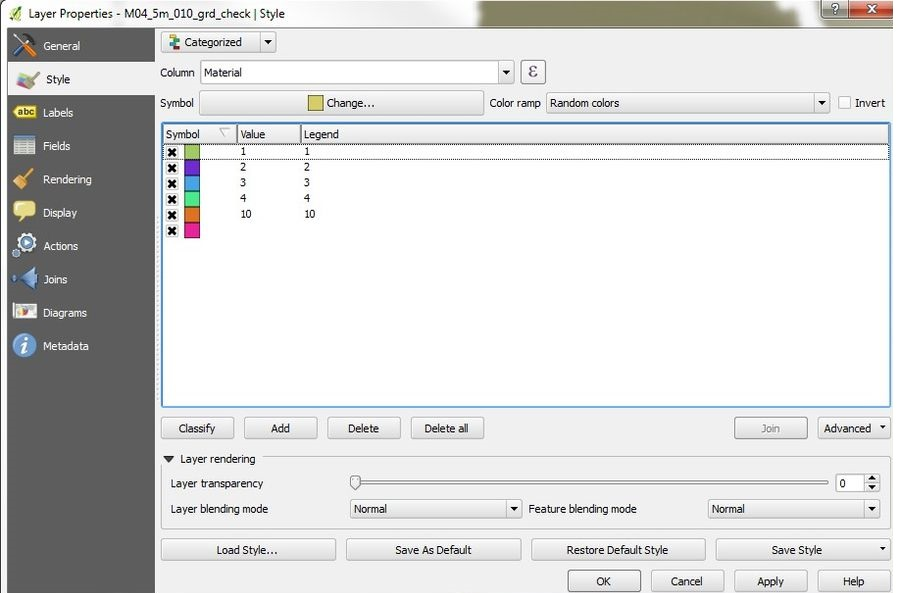
\includegraphics[width=0.52\textwidth]{images/qGisUi.jpg} 
\end{center} \vspace{-20pt} \caption{Interfaz visual QGis.}  \label{qGisvisual} \vspace{-10pt} 
\end{wrapfigure}

Tampoco se puede integrar al proyecto OLS con facilidad debido a que est\'a en otro lenguaje y, para a\~nadirlo, habr\'ia que migrar todo el c\'odigo a C-sharp, que ser\'ia tan o m\'as costoso que implementar la herramienta de mapas tem\'aticos desde cero, adem\'as, esto no garantizar\'a que la migraci\'on quede libre de errores. Tambi\'en se puede decir que esta herramienta no permite realizar restricciones sobre una misma capa para tematizar la informaci\'on de esta. Por \'ultimo, a pesar de que existen \emph{bindings} \footnote{adaptaci\'on de una biblioteca para ser usada en un lenguaje de programaci\'on distinto de aquel en el que ha sido escrita. Esta palabra no tiene traducci\'on al espa\~nol} de la librer\'ia Qt de interfaz de usuario para C-sharp, se dificulta su uso por la misma problem\'atica de la migraci\'on de c\'odigo, sin dejar de mencionar que es necesario modificar, por no decir, cambiar por completo el c\'odigo de la interfaz, puesto que el manejo de la configuraci\'on de QGis se diferencia, en gran medida, con la de OLS, osea que no podemos integrar directamente el frontend al servidor, sino que se tiene que adaptar, en cuyo caso es preferible hacer una interfaz propia con un framework que se ajuste a las necesidades de OLS.


\subsection{ArcGis}
ArcGis es un completo sistema que permite recopilar, organizar, administrar, analizar, compartir y distribuir informaci\'on geogr\'afica. Permite crear y utilizar Sistemas de Informaci\'on Geogr\'afica. Una de las principales funcionalidades de ArcGIS es la creaci\'on y dise\~no de cartograf\'ia. Los mapas generados pueden ser de diversa tipolog\'ia, siendo una de las m\'as destacadas la de mapas tem\'aticos (figura \ref{arcGis}). Estos mapas permiten captar el inter\'es de los usuarios y proporcionarles informaci\'on de forma muy visual, ofreciendo un m\'etodo ideal para mostrar los resultados del trabajo SIG.

\begin{wrapfigure}{l}{0.5\textwidth}
\vspace{-20pt}
\begin{center}
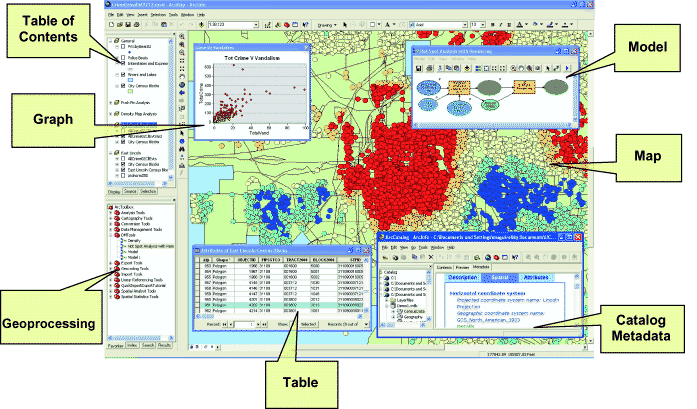
\includegraphics[width=0.52\textwidth]{images/arcGis.png} 
\end{center} \vspace{-20pt} \caption{ArcGis. Interfaz visual y mapa tem\'atico.}  \label{arcGis} \vspace{-10pt} 
\end{wrapfigure}

Las ventajas que presenta esta herramienta radican en que proporciona una amplia posibilidad de recursos relacionados con los mapas tem\'aticos. Con esta herramienta se pueden crear, consultar y analizar datos; combinar varias capas; aplicar funciones matem\'aticas, construir y obtener nueva informaci\'on a partir de tem\'aticos ya existentes, etc. En ArcGis, la finalidad de un mapa tem\'atico es la de representar de una o varias caracter\'isticas de fen\'omenos geogr\'aficos, pudiendo dividir a estos en objetos reales: distribuci\'on, densidad, relaci\'on, etc; y conceptos abstractos: indicadores de desarrollo econ\'omico, calidad de vida, etc. Estos mapas pueden ser publicados en web permitiendo, mediante ventanas emergentes, la visualizaci\'on de una o varias de estas caracter\'isticas,  fotograf\'ias de los fen\'omenos y acceso a otra informaci\'on en la web. \cite{ART} 

La principal desventaja que presenta este software es que no es c\'odigo abierto, sino que se distribuye comercialmente bajo tres niveles de licencia, por lo tanto se descarta por no ser de c\'odigo abierto y no ser gratuito. Adem\'as, la interfaz de usuario que presenta es un poco complicada, debido a que cada documento diferente en ArcGIS utiliza una GUI separada, cada GUI se compone por barra de botones, herramientas, men\'us, estados y l\'ineas de comando, lo que dificulta su uso por usuarios poco preparados, y no es lo que se quiere en OLS.


\subsection{MapInfo}
Las soluciones que proporciona MapInfo \cite{mapinfo} para la creaci\'on de mapas permiten llevar a cabo an\'alisis geogr\'aficos sencillos y complejos, acceso a datos remotos y creaci\'on de mapas tem\'aticos que revelen patrones en los datos. Se pueden visualizar los datos como puntos, regiones zonificadas tem\'aticamente, como gr\'aficos de tartas o de barras , etc.

\begin{wrapfigure}{l}{0.5\textwidth}
\vspace{-20pt}
\begin{center}
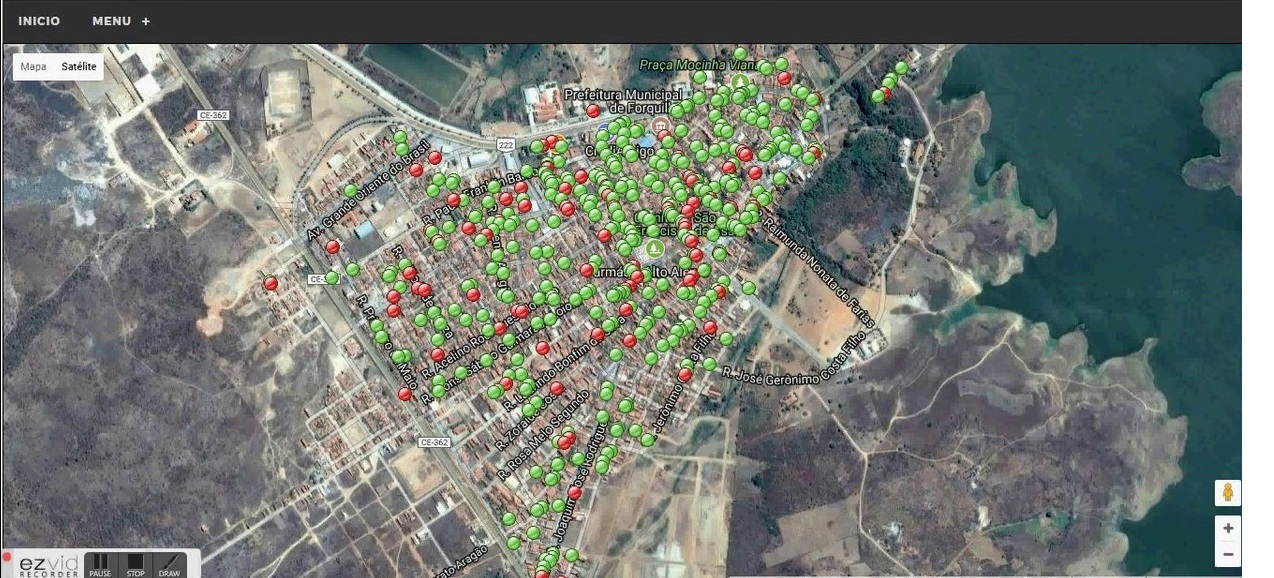
\includegraphics[width=0.52\textwidth]{images/mapInfoTematic.jpg} 
\end{center} \vspace{-20pt} \caption{Mapa tem\'atico creado con MapInfo.}  \label{mapinfo} \vspace{-10pt} 
\end{wrapfigure}

Como parte de las caracter\'isticas ventajosas se encuentran que, con MapInfo, se pueden crear distintos mapas tem\'aticos asign\'andoles a estos colores, patrones o s\'imbolos para establecer una coincidencia con objetos seg\'un valores espec\'ificos de la tabla. La caracter\'istica Mapa tem\'atico utiliza un asistente compuesto de una secuencia de tres cuadros de di\'alogo que facilitan la selecci\'on del tipo de mapa tem\'atico que se desea, las tablas y los campos que se utilizar\'an para construir el mapa y diversas opciones para personalizarlo. Las plantillas tem\'aticas de MapInfo facilitan el comienzo de la creaci\'on de un tema. Se selecciona una plantilla que represente el tipo de mapa tem\'atico que se desea. Las plantillas se pueden personalizar completamente y pueden guardarse como nuevas plantillas en caso de que se precisen para la creaci\'on de mapas tem\'aticos m\'as adelante. Con MapInfo se suministran m\'as de 40 plantillas. MapInfo cuenta con una potente y flexible interfaz de usuario, interactiva para mapas tem\'aticos, esta interfaz permite a los usuarios anclar las barras de herramientas en los cuatro lados de la aplicaci\'on, ayudando a mejorar la eficiencia, reducir la conglomeraci\'on sobre la pantalla, y ahorrar tiempo. \cite{mapinfo}

\begin{wrapfigure}{l}{0.5\textwidth}
\vspace{-20pt}
\begin{center}
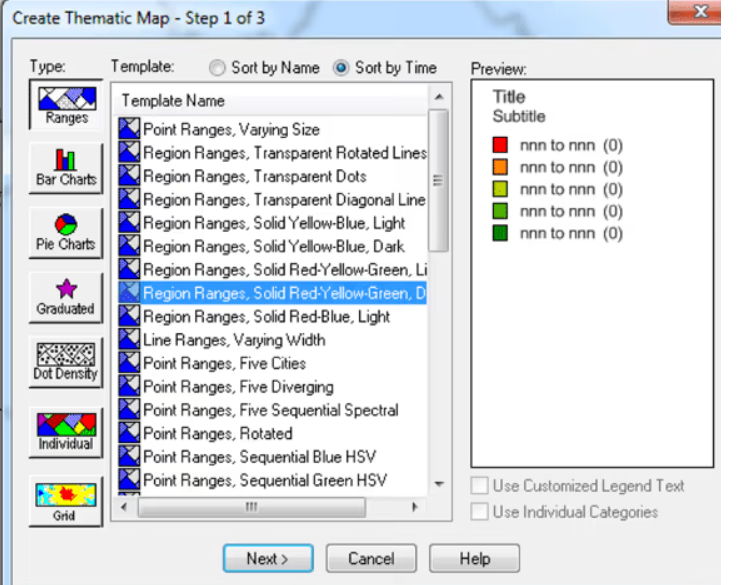
\includegraphics[width=0.52\textwidth]{images/mapInfoUi.png} 
\end{center} \vspace{-20pt} \caption{Interfaz visual de configuraci\'on de MapInfo.}  \label{mapinfo2} \vspace{-10pt} 
\end{wrapfigure}

Como parte de las desventajas que nos inclinan a descartar a MapInfo se encuentra que no es multiplataforma, solo est\'a disponible para Windows\footnote{sistema operativo, es decir, un conjunto de programas que posibilita la administraci\'on de los recursos de una computadora}. Adem\'as, es un software privado de la compa\~n\'ia Precisely, antiguamente Pitney Bowes Inc, lo que no se corresponde con las pol\'iticas de migraci\'on a software libre e imposibilita su adquisici\'on. Finalmente, es un software basado en Python\footnote{lenguaje de programaci\'on ampliamente utilizado en las aplicaciones web, el desarrollo de software, la ciencia de datos y el machine learning}, lo cual entorpecer\'ia su integraci\'on a OLS por la problem\'atica antes mencionada de migraci\'on de c\'odigo.


\subsection{SharpMap}
SharpMap \cite{sharpmap} es una biblioteca de clases para crear aplicaciones web. Con esta librer\'ia se pueden realizar consultas a los datos espaciales para el manejo y an\'alisis de los mismos.

\begin{wrapfigure}{l}{0.5\textwidth}
\vspace{-20pt}
\begin{center}
\includegraphics[width=0.52\textwidth]{images/sharpmap.png} 
\end{center} \vspace{-20pt} \caption{Mapa tem\'atico creado con SharpMap.}  \label{sharpmap} \vspace{-10pt} 
\end{wrapfigure}

Ser\'ia ventajoso el uso de SharMap ya que es un sistema SIG escrito totalmente en C\# .NET 4.0, y admite m\'ultiples lenguajes de desarrollo .Net (C\#, C$++$, etc). Tambi\'en, presenta la clase \textit{CustomTheme}, que es usada para definir un tem\'atico propio, esta presenta dos m\'etodos p\'ublicos: \textit{CustomTheme}, para crear la clase, y \textit{GetStyle}, para obtener un estilo para pintar el tem\'atico. Adem\'as, con la herramienta \textit{SharpMap.Rendering.Thematics.CategoryTheme} se crean categor\'ias usando rangos de valores para comparar con el campo elegido. \cite{sharpmap}

Una notale desventaja de esta biblioteca es que al no ser multiplataforma dar\'ia un paso atr\'as en el desarrollo de OLS, que ya
fue mejorado a un proyecto multiplataforma. Por otro lado, al estar basado en el framework .Net 4.0, y este no presentar una versi\'on compatible con ASP.NET Core, entra en conflicto con la \'ultima versi\'on de OLS, que ya fue migrado a ASP.NET Core. SharpMap carece, adem\'as, de una interfaz visual, por lo que es necesario usar c\'odigo, lo cual dificulta a usuarios que no est\'en familiarizados con la programaci\'on hacer uso de esta, y es una de las cosas que se quiere evitar en OLS. Por \'ultimo, otra restricci\'on que presenta esta biblioteca, es que no presenta muchos tipos de tem\'aticos.


\section{Frameworks y librer\'ias de JavaScript que se pueden utilizar en la interfaz visual de OLS.}

Como se dijo anteriormente, se hace necesario la creaci\'on de una interfaz propia que responda a las necesidades particulares de OLS. Los Frameworks de interfaz gr\'afica son soluciones completas que contemplan herramientas de apoyo a la construcci\'on de software para la capa de presentaci\'on, brindando al usuario aplicaciones atractivas. Las bibliotecas, y los marcos de trabajo de JavaScript\footnote{lenguaje de programaci\'on que se utiliza para hacer p\'aginas web interactivas}, facilitan el desarrollo de sitios web y aplicaciones con caracter\'isticas y funcionalidades muy variadas, todo ello gracias a las caracter\'isticas din\'amicas, flexibles y atractivas de JavaScript. Seg\'un una encuesta de StackOverflow\footnote{sitio de preguntas y respuestas para desarrolladores dise\~nado para resolver problemas y aprender} de 2020, JavaScript sigue siendo el lenguaje de programaci\'on m\'as utilizado (por octavo a\~no), con un 67,7\% de los encuestados que lo utilizan. Su versatilidad favorece el desarrollo del front-end, adem\'as de las pruebas. Como resultado, se pueden encontrar muchas bibliotecas y frameworks de JavaScript que sirven para varios prop\'ositos. En el mercado existe una amplia gama de Frameworks y librer\'ias que proveen soluciones para el desarrollo de aplicaciones web, y la creaci\'on de interfaces gr\'aficas. En este ep\'igrafe se estudiar\'an aquellos que, por sus caracter\'isticas y su uso en el mundo de la programaci\'on web, se consideran m\'as importantes.


\subsection{React}
ReactJS (figura \ref{react}) es una librer\'ia escrita en JavaScript de c\'odigo abierto enfocada a la visualizaci\'on para facilitar la creaci\'on de componentes interactivos y reutilizables para interfaces de usuario \cite{react}. Esta librer\'ia fue lanzada en el a\~no 2013 y desarrollada por Facebook, quienes tambi\'en la mantienen actualmente junto a una comunidad de desarrolladores independientes y compa\~n\'ias. 

\begin{wrapfigure}{l}{0.5\textwidth}
\vspace{-20pt}
\begin{center}

\includegraphics[width=0.52\textwidth]{images/reactLogo.png} 
\end{center} \vspace{-20pt} \caption{Logo React.}  \label{react} \vspace{-10pt} 
\end{wrapfigure}

La caracter\'istica m\'as importante de ReactJS es el componente, una pieza de interfaz de usuario. Al dise\~nar una App con React, lo que se crean son componentes independientes y reusables para crear interfaces de usuario m\'as complejas. De esta manera, ReactJS est\'a basado en un paradigma llamado programaci\'on orientada a componentes en el que cada componente es una pieza con la que el usuario puede interactuar. Estas piezas se crean usando una sintaxis llamada JSX \cite{react} permitiendo escribir HTML\footnote{lenguaje con el que se define el contenido de las p\'aginas web} (y opcionalmente CSS\footnote{lenguaje que maneja el dise\~no y presentaci\'on de las p\'aginas web}) dentro de objetos JavaScript.

Entre las muchas ventajas que tiene el uso de React resalta el desarrollo rentable, ofreciendo una v\'ia econ\'omica para crear aplicaciones multiplataforma. Adem\'as, se necesitan menos esfuerzos, ya que se requiere menos c\'odigo en comparaci\'on con otras plataformas de desarrollo. Tambi\'en, dado el hecho de que ReactJS es una plataforma de c\'odigo abierto con licencia del MIT, brinda acceso para usar bibliotecas y marcos de forma gratuita.

Como parte de las desventajas que motivaron a no usar esta biblioteca se destacan la ausencia de documentaci\'on oficial. La alta velocidad de desarrollo de ReactJS apenas deja lugar a una documentaci\'on apropiada, la cual es algo ca\'otica ya que diferentes desarrolladores contribuyen sin un enfoque com\'un. Por otro lado, no existe un est\'andar de desarrollo, de modo que tenemos demasiadas elecciones a tomar. Adem\'as, el alto ritmo de desarrollo de esta herramienta, provoca volver a aprender nuevas formas de hacer las cosas regularmente, cada vez que se realizan nuevos cambios, y resulta dif\'icil para los desarrolladores adoptar todos los cambios con todas las actualizaciones continuas. Por \'ultimo, la integraci\'on de React con un marco MVC\footnote{Modelo Vista Controlador, estilo de arquitectura de software que separa los datos de una aplicaci\'on, la interfaz de usuario, y la l\'ogica de negocio en tres componentes distintos} como nuestro servidor requiere una gran cantidad de configuraci\'on.


\subsection{Vue}
Vue (figura \ref{vue}) es un marco de trabajo flexible y ligero basado en JavaScript que ofrece potentes herramientas web para desarrollar proyectos web frontales modernistas \cite{vue}. Vue tambi\'en se considera un marco JavaScript flexible y evolutivo, ya que permite realizar cambios en el c\'odigo de una aplicaci\'on sin que ello afecte a ninguna caracter\'istica fundamental, lo que permite crear una interfaz de usuario progresiva. La gran flexibilidad de Vue tambi\'en permite a\~nadir m\'odulos a medida y componentes visuales a la funcionalidad de la aplicaci\'on web.

\begin{wrapfigure}{l}{0.5\textwidth}
\vspace{-20pt}
\begin{center}

\includegraphics[width=0.52\textwidth]{images/vueLogo.png} 
\end{center} \vspace{-20pt} \caption{Logo Vue.}  \label{vue} \vspace{-10pt} 
\end{wrapfigure}

Como parte de las ventajas de esta herramienta podemos mencionar que presenta HTML empoderado, esto significa que Vue.js tiene muchas similitudes con Angular, y esto puede ayudar a optimizar el manejo de bloques HTML usando diferentes componentes. Por otro lado, tiene una documentaci\'on muy completa, que puede acelerar la curva de aprendizaje para desarrolladores y ahorrar mucho tiempo en el desarrollo de una aplicaci\'on, usando s\'olo conocimientos b\'asicos de HTML y JavaScript. Se puede decir, adem\'as, que este framework se usa para construir tanto aplicaciones de p\'agina \'unica (SPA)\footnote{aplicaciones o sitios web que cargan todos los recursos necesarios para navegar por los sitios web en la primera carga de la p\'agina} o complejas interfaces web de aplicaciones. Tambi\'en, Vue.js puede ocupar cerca de 20KB manteniendo su velocidad y flexibilidad, que permite alcanzar un mejor rendimiento en comparaci\'on con otros frameworks. Finalmente, Vue.js ayuda a construir grandes plantillas reutilizables en poco tiempo de acuerdo con su sencilla estructura.

Como desventaja, Vue.js a\'un tiene poca cuota de mercado comparado con Angular o React, lo que significa que los recursos disponibles de este framework a\'un est\'an en su fase inicial. Por otra parte, su gran flexibilidad puede ser un contratiempo, puesto que, en ocasiones, Vue.js puede tener problemas para integrarse en grandes proyectos y a\'un no hay experiencia acerca de posibles soluciones. La barrera del idioma es un contra de esta herramienta ya que el creador es en realidad chino-estadounidense y apoya mucho a la comunidad de desarrollo china. La mayor\'ia de los usuarios son comunidades de habla no inglesa, que son quiz\'as uno de los mayores problemas con este marco. Predominantemente, la mayor parte de la codificaci\'on est\'a escrita en chino, esto complica el trabajo de los desarrolladores de habla inglesa con Vue.js. Por estas razones se ha desestimado el uso de este framework.


\subsection{Angular}
Angular (figura \ref{angular}) es una plataforma de desarrollo, construida sobre TypeScript\footnote{lenguaje de programaci\'on construido a un nivel superior de JavaScript, que a\~nade tipados est\'aticos y objetos basados en clases}, un framework basado en componentes para crear aplicaciones web escalables. Es una colecci\'on de bibliotecas bien integradas que cubren una amplia variedad de caracter\'isticas, que incluyen enrutamiento, administraci\'on de formularios, comunicaci\'on cliente-servidor y m\'as \cite{angular}.

Angular proporciona un conjunto de herramientas que permiten desarrollar, compilar, probar y actualizar el c\'odigo fuente de la aplicaci\'on. Se ha convertido en una alternativa popular para dise\~nar aplicaciones multiplataforma ya que admite arquitecturas MVC y MVVM\footnote{patr\'on Model-View-ViewModel, ayuda a separar limpiamente la l\'ogica empresarial y de presentaci\'on de una aplicaci\'on de su interfaz de usuario} del lado del cliente, lo que facilita a los desarrolladores la creaci\'on de aplicaciones.

\begin{wrapfigure}{l}{0.5\textwidth}
\vspace{-20pt}
\begin{center}

\includegraphics[width=0.52\textwidth]{images/angularLogo.png} 
\end{center} \vspace{-20pt} \caption{Logo Angular.}  \label{angular} \vspace{-10pt} 
\end{wrapfigure}

Como ventajas, se puede decir que Angular tiene una estructura basada en componentes lo que hace que estos sean altamente reutilizables, y simplifica el proceso de desarrollo. Angular tiene, adem\'as, una gu\'ia de estilo de documentaci\'on y CLI\footnote{herramienta de l\'inea de comandos que se utiliza para inicializar, desarrollar, estructurar y mantener aplicaciones de Angular}, ambas consistencias de unidad. La codificaci\'on consistente tiene varios beneficios como plantillas o fragmentos predefinidos, f\'acil uso de sitios, etc. Tambi\'en, es compatible con arquitectura MVC, y utiliza la fuente HTML para describir la interfaz de usuario de la aplicaci\'on porque es un lenguaje intuitivo, declarativo y menos complicado. Por \'ultimo, cuando se implementa para proyectos de desarrollo web, Angular se integra sin problemas, ofreciendo un marco inteligente y robusto que ahorra mucho tiempo a los desarrolladores. 

Este framework tambi\'en presenta desventajas, entre las que pueden mencionarse su sintaxis compleja, heredada de la primera versi\'on de Angular. Aunque Angular usa TypeScript, que es menos dif\'icil de aprender. Tambi\'en, pueden aparecer problemas con la migraci\'on de anteriores versiones pero, si se usa en OLS, no ser\'an necesarias estas migraciones.

Seg\'un el an\'alisis de las ventajas y desventajas realizadas en este ep\'igrafe, se decide hacer uso del framework Angular para desarrollar la interfaz visual de configuraci\'on de OLS.


\section{Conclusiones}
A lo largo de este cap\'itulo se analizaron varios Sistemas de Informaci\'on Geogr\'afica que implementan mapas tem\'aticos. Se estudiaron QGis, ArcGis, MapInfo y SharpMap. Los cuales presentan deficiencias si se integran a OLS, entre las causas comunes que llevaron a su desestimaci\'on se encuentran que la mayor\'ia de estas herramientas est\'an en otros lenguajes no compatibles con los del servidor OLS, por lo que ser\'ia igual, o m\'as complicado, su migraci\'on a OLS, que desarrollar una herramienta propia desde cero, la excepci\'on a esta desventaja la presenta SharpMap, pero se descart\'o debido a que no es multiplataforma y su versi\'on de .Net Core no es la misma de OLS, adem\'as de no presentar una interfaz visual. Otras complicaciones que se analizaron fueron la poca capacidad para generar tem\'aticos, como es el caso de QGis, donde, adem\'as, su interfaz visual est\'a implementada en otro lenguaje de programaci\'on. Por otro lado, ArcGis no es de c\'odigo abierto y no es gratuito, y tambi\'en esta herramienta presenta una interfaz de usuario compleja. Finalmente, a pesar de que MapInfo presenta una potente y flexible interfaz de usuario y funcionalidades \'utiles para tem\'aticos, se descarta por no ser multiplataforma y ser un software privado.

Por los motivos antes expuestos, se llega a la conclusi\'on de que la mejor opci\'on es implementar una nueva herramienta que permita configurar y visualizar mapas tem\'aticos de clasificaci\'on de tipos.

En el segundo ep\'igrafe, se analizaron ventajas y desventajas de frameworks y librer\'ias de JavaScript con el objetivo de seleccionar uno para implementar la interfaz visual de OLS. Se analizaron React, Vue y Angular como marcos de trabajo. Se pudo observar que React y Vue no son tan estructurados y definidos como puede ser Angular. React, adem\'as, no cuenta con una fuerte documentaci\'on oficial y necesita mucha configuraci\'on para integrarlo a proyectos como OLS. Vue, a pesar de que est\'a ganando popularidad, no cuenta con un fuerte apoyo de la comunidad de programadores como React o Angular, por otro lado, a pesar de tener una gran documentaci\'on, esta est\'a en su mayor\'ia en chino, lo que dificulta su aprendizaje. Finalmente, debido a que Angular esta basado en TypeScript, su modularidad y jerarqu\'ia de componentes, adem\'as del excelente soporte de la comunidad y de Google, entre otras ventajas previamente expuestas, se decide usar este framework para implementar la interfaz visual de OLS.
